% =============================================================================
% Professional Beamer Presentation Template
% PhD Survival Kit — Prof. Milan Amrut Joshi
% =============================================================================
%
% USAGE:
%   pdflatex template.tex
%
% FEATURES:
%   - 16:9 widescreen aspect ratio
%   - Custom professional blue/purple color scheme
%   - Speaker notes enabled (compile with \setbeameroption{show notes on second screen})
%   - Math, figures, tables, and code block examples
%
% =============================================================================

\documentclass[aspectratio=169, 11pt]{beamer}

% =============================================================================
% THEME AND COLORS
% =============================================================================

% --- Base Theme ---
\usetheme{Madrid}
\useinnertheme{circles}     % Bullet style
\useoutertheme{default}

% --- Custom Color Scheme: Professional Blue/Purple ---
\definecolor{PrimaryBlue}{RGB}{25, 55, 109}     % Deep navy blue
\definecolor{AccentPurple}{RGB}{102, 51, 153}    % Rich purple
\definecolor{LightBlue}{RGB}{218, 232, 252}      % Light blue for backgrounds
\definecolor{DarkText}{RGB}{33, 33, 33}           % Near-black for body text
\definecolor{CodeBg}{RGB}{245, 245, 250}          % Light gray for code blocks
\definecolor{HighlightGreen}{RGB}{39, 174, 96}    % Green for emphasis

\setbeamercolor{palette primary}{bg=PrimaryBlue, fg=white}
\setbeamercolor{palette secondary}{bg=AccentPurple, fg=white}
\setbeamercolor{palette tertiary}{bg=PrimaryBlue!80!black, fg=white}
\setbeamercolor{palette quaternary}{bg=PrimaryBlue, fg=white}
\setbeamercolor{structure}{fg=PrimaryBlue}
\setbeamercolor{title}{fg=white, bg=PrimaryBlue}
\setbeamercolor{frametitle}{fg=white, bg=PrimaryBlue}
\setbeamercolor{block title}{bg=PrimaryBlue, fg=white}
\setbeamercolor{block body}{bg=LightBlue, fg=DarkText}
\setbeamercolor{block title alerted}{bg=red!70!black, fg=white}
\setbeamercolor{block body alerted}{bg=red!10, fg=DarkText}
\setbeamercolor{block title example}{bg=HighlightGreen!80!black, fg=white}
\setbeamercolor{block body example}{bg=HighlightGreen!10, fg=DarkText}
\setbeamercolor{item}{fg=PrimaryBlue}
\setbeamercolor{section in toc}{fg=PrimaryBlue}

% --- Font Configuration ---
\setbeamerfont{title}{size=\Large, series=\bfseries}
\setbeamerfont{subtitle}{size=\normalsize}
\setbeamerfont{frametitle}{size=\large, series=\bfseries}
\setbeamerfont{framesubtitle}{size=\small}
\setbeamerfont{footnote}{size=\tiny}

% --- Remove navigation symbols (they clutter the slides) ---
\setbeamertemplate{navigation symbols}{}

% --- Show slide numbers in footer ---
\setbeamertemplate{footline}{
    \leavevmode%
    \hbox{%
        \begin{beamercolorbox}[wd=.333333\paperwidth,ht=2.25ex,dp=1ex,center]{author in head/foot}%
            \usebeamerfont{author in head/foot}\insertshortauthor
        \end{beamercolorbox}%
        \begin{beamercolorbox}[wd=.333333\paperwidth,ht=2.25ex,dp=1ex,center]{title in head/foot}%
            \usebeamerfont{title in head/foot}\insertshorttitle
        \end{beamercolorbox}%
        \begin{beamercolorbox}[wd=.333333\paperwidth,ht=2.25ex,dp=1ex,right]{date in head/foot}%
            \usebeamerfont{date in head/foot}\insertshortdate{}\hspace*{2em}
            \insertframenumber{} / \inserttotalframenumber\hspace*{2ex}
        \end{beamercolorbox}%
    }%
    \vskip0pt%
}

% =============================================================================
% PACKAGES
% =============================================================================

\usepackage{amsmath, amssymb}    % Math
\usepackage{graphicx}            % Figures
\usepackage{booktabs}            % Professional tables
\usepackage{hyperref}            % Links
\usepackage{listings}            % Code blocks
\usepackage{tikz}                % Diagrams
\usepackage{multimedia}          % Video embedding (optional)
\usepackage{appendixnumberbeamer}% Correct numbering for backup slides

% --- Code Block Styling ---
\lstset{
    language=Python,
    basicstyle=\ttfamily\footnotesize,
    keywordstyle=\color{PrimaryBlue}\bfseries,
    stringstyle=\color{HighlightGreen},
    commentstyle=\color{gray}\itshape,
    numbers=left,
    numberstyle=\tiny\color{gray},
    numbersep=5pt,
    backgroundcolor=\color{CodeBg},
    frame=single,
    rulecolor=\color{gray!30},
    breaklines=true,
    showstringspaces=false,
    tabsize=4,
}

% --- Speaker Notes Configuration ---
% Uncomment the next line to show notes on a second screen:
% \setbeameroption{show notes on second screen=right}
\setbeamertemplate{note page}{%
    \insertnote%
}

% =============================================================================
% TITLE PAGE INFORMATION
% =============================================================================

\title[Short Title]{Full Presentation Title}
\subtitle{Subtitle or Conference/Venue Name}
\author[M.A. Joshi]{%
    \textbf{Milan Amrut Joshi}\inst{1} \and
    Coauthor Name\inst{2}
}
\institute[University]{%
    \inst{1} Department of Computer Science, University Name \and
    \inst{2} Department of Engineering, Other University
}
\date[CONF 2026]{International Conference on XYZ \\ February 22, 2026}
% \titlegraphic{\includegraphics[height=1cm]{figures/university_logo.png}}

% =============================================================================
% DOCUMENT
% =============================================================================
\begin{document}

% ----- TITLE SLIDE -----
\begin{frame}[plain]
    \titlepage
    \note{
        Welcome everyone. Thank you for attending this talk.
        Today I will present our work on [topic].
        This is joint work with [coauthor] from [institution].
    }
\end{frame}

% ----- OUTLINE SLIDE -----
\begin{frame}{Outline}
    \tableofcontents
    \note{
        Here is an overview of the talk.
        I will start with motivation, then move to our approach,
        show experimental results, and conclude with future directions.
    }
\end{frame}

% =============================================================================
% SECTION 1: INTRODUCTION / MOTIVATION
% =============================================================================
\section{Introduction}

\begin{frame}{Motivation}
    \begin{columns}[T]
        \begin{column}{0.55\textwidth}
            \textbf{Why does this problem matter?}
            \begin{itemize}
                \item First motivation point with context
                \item Second point explaining real-world impact
                \item Third point establishing urgency
            \end{itemize}

            \vspace{0.5em}
            \textbf{Key Challenge:}
            \begin{alertblock}{Problem Statement}
                Concisely state the specific problem your work addresses.
            \end{alertblock}
        \end{column}
        \begin{column}{0.40\textwidth}
            % Replace with your figure:
            % \includegraphics[width=\textwidth]{figures/motivation.pdf}
            \begin{block}{Placeholder}
                \centering
                \vspace{2cm}
                [Motivating Figure]
                \vspace{2cm}
            \end{block}
        \end{column}
    \end{columns}
    \note{
        Start by explaining WHY the audience should care.
        Connect to a real-world problem they can relate to.
        Spend about 2 minutes on this slide.
    }
\end{frame}

\begin{frame}{Background}
    \begin{block}{Definition (Key Concept)}
        Let $\mathcal{X}$ be a topological space. A \textbf{persistent homology}
        is a sequence of homology groups connected by homomorphisms induced
        by inclusion maps.
    \end{block}

    \vspace{1em}

    \textbf{Key properties:}
    \begin{enumerate}
        \item Property one with mathematical notation: $H_k(\mathcal{X})$
        \item Property two: captures multi-scale features
        \item Property three: stable under perturbations
    \end{enumerate}

    \note{
        Provide just enough background for the audience to follow your talk.
        Do not over-explain known concepts.
        Adjust based on audience expertise level.
    }
\end{frame}

% =============================================================================
% SECTION 2: METHODOLOGY
% =============================================================================
\section{Proposed Approach}

\begin{frame}{Method Overview}
    \centering
    % Architecture diagram using TikZ
    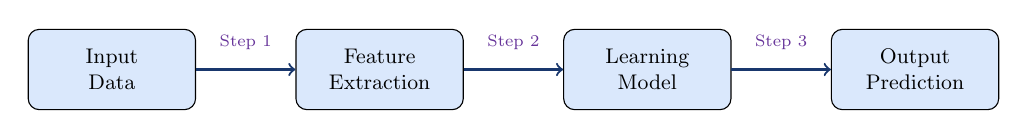
\begin{tikzpicture}[
        box/.style={draw, rounded corners, fill=LightBlue,
                     minimum height=1.2cm, minimum width=2.5cm,
                     font=\small, align=center},
        arrow/.style={->, thick, PrimaryBlue},
        scale=0.85, transform shape
    ]
        \node[box] (input) at (0,0) {Input\\Data};
        \node[box] (feat) at (4,0) {Feature\\Extraction};
        \node[box] (model) at (8,0) {Learning\\Model};
        \node[box] (output) at (12,0) {Output\\Prediction};

        \draw[arrow] (input) -- (feat);
        \draw[arrow] (feat) -- (model);
        \draw[arrow] (model) -- (output);

        \node[font=\scriptsize, AccentPurple] at (2, 0.4) {Step 1};
        \node[font=\scriptsize, AccentPurple] at (6, 0.4) {Step 2};
        \node[font=\scriptsize, AccentPurple] at (10, 0.4) {Step 3};
    \end{tikzpicture}

    \vspace{1em}
    \begin{itemize}
        \item \textbf{Step 1:} Extract topological features from input data
        \item \textbf{Step 2:} Learn representations using proposed method
        \item \textbf{Step 3:} Produce final predictions
    \end{itemize}

    \note{
        Walk through the pipeline left to right.
        This is the key slide for understanding your method.
        Spend 3-4 minutes here.
    }
\end{frame}

\begin{frame}{Mathematical Formulation}
    Given dataset $\mathcal{D} = \{(x_i, y_i)\}_{i=1}^{n}$, we minimize:

    \begin{equation*}
        \mathcal{L}(\theta) = \underbrace{\frac{1}{n}\sum_{i=1}^{n}
        \ell(f_\theta(x_i), y_i)}_{\text{empirical risk}}
        + \underbrace{\lambda \|\theta\|_2^2}_{\text{regularization}}
    \end{equation*}

    \vspace{0.5em}
    where:
    \begin{itemize}
        \item $f_\theta: \mathbb{R}^d \to \mathbb{R}^k$ is the model
        \item $\ell(\cdot, \cdot)$ is the cross-entropy loss
        \item $\lambda > 0$ controls regularization strength
    \end{itemize}

    \begin{exampleblock}{Key Insight}
        Our approach differs from prior work by incorporating
        topological features directly into the loss function,
        enabling structure-aware learning.
    \end{exampleblock}

    \note{
        Keep math slides focused on ONE key equation.
        Explain each term clearly. Do not rush through notation.
    }
\end{frame}

% =============================================================================
% SECTION 3: EXPERIMENTS
% =============================================================================
\section{Experiments}

\begin{frame}{Experimental Setup}
    \begin{columns}[T]
        \begin{column}{0.48\textwidth}
            \textbf{Datasets:}
            \begin{table}
                \centering
                \footnotesize
                \begin{tabular}{lcc}
                    \toprule
                    \textbf{Dataset} & \textbf{Size} & \textbf{Classes} \\
                    \midrule
                    MNIST      & 70K  & 10  \\
                    CIFAR-10   & 60K  & 10  \\
                    ImageNet   & 1.2M & 1000 \\
                    \bottomrule
                \end{tabular}
            \end{table}
        \end{column}
        \begin{column}{0.48\textwidth}
            \textbf{Implementation:}
            \begin{itemize}
                \item Python 3.10 + PyTorch 2.0
                \item NVIDIA RTX 3090 GPU
                \item Adam optimizer, $\eta = 10^{-3}$
                \item Batch size: 64
                \item 100 epochs, early stopping
            \end{itemize}
        \end{column}
    \end{columns}

    \note{
        Briefly cover the setup. Audience mainly cares about results.
        Be ready to answer detailed questions about hyperparameters.
    }
\end{frame}

\begin{frame}{Results --- Comparison with State of the Art}
    \begin{table}
        \centering
        \begin{tabular}{lcccc}
            \toprule
            \textbf{Method} & \textbf{Acc.} & \textbf{Prec.} & \textbf{Rec.} & \textbf{F1} \\
            \midrule
            Baseline A       & 91.2 & 90.8 & 91.0 & 90.9 \\
            Baseline B       & 92.5 & 92.1 & 92.3 & 92.2 \\
            Baseline C       & 93.1 & 91.9 & 93.0 & 92.4 \\
            \midrule
            \rowcolor{LightBlue}
            \textbf{Ours}    & \textbf{94.3} & \textbf{94.0} & \textbf{94.1} & \textbf{94.0} \\
            \bottomrule
        \end{tabular}
        \caption{Results on Dataset A. Bold = best.}
    \end{table}

    \vspace{0.5em}
    \begin{itemize}
        \item \textcolor{HighlightGreen}{\textbf{+1.2\%}} accuracy improvement over best baseline
        \item Consistent gains across all evaluation metrics
        \item Statistically significant ($p < 0.01$, paired $t$-test)
    \end{itemize}

    \note{
        This is the MOST IMPORTANT slide. Highlight key numbers.
        Point to specific rows in the table while presenting.
        Be prepared to explain why your method performs better.
    }
\end{frame}

% =============================================================================
% SECTION 4: CODE EXAMPLE (optional)
% =============================================================================
\section{Implementation}

\begin{frame}[fragile]{Code Example}
    \begin{lstlisting}[caption={Core implementation in PyTorch}]
import torch
import torch.nn as nn

class TopologicalLayer(nn.Module):
    def __init__(self, in_dim, out_dim):
        super().__init__()
        self.linear = nn.Linear(in_dim, out_dim)
        self.activation = nn.ReLU()

    def forward(self, x, persistence):
        # Combine standard features with
        # topological persistence features
        topo_feat = self.compute_topo(persistence)
        combined = torch.cat([x, topo_feat], dim=-1)
        return self.activation(self.linear(combined))
    \end{lstlisting}

    \note{
        Show code only if the audience is technical and implementation
        details add value. Keep it short and highlight the key parts.
    }
\end{frame}

% =============================================================================
% SECTION 5: CONCLUSION
% =============================================================================
\section{Conclusion}

\begin{frame}{Summary and Future Work}
    \textbf{Summary:}
    \begin{itemize}
        \item We proposed [method name] for [problem]
        \item Key innovation: [one sentence]
        \item Achieves state-of-the-art results on [N] benchmarks
    \end{itemize}

    \vspace{1em}
    \textbf{Future Directions:}
    \begin{enumerate}
        \item Extend to [larger scale / different domain]
        \item Investigate [theoretical analysis / interpretability]
        \item Apply to [real-world application]
    \end{enumerate}

    \vspace{1em}
    \begin{block}{Resources}
        \centering
        Code: \url{https://github.com/username/project} \\
        Paper: \url{https://arxiv.org/abs/XXXX.XXXXX}
    \end{block}

    \note{
        Summarize in 3 bullet points. Leave the audience with a clear
        takeaway message. Transition smoothly to questions.
    }
\end{frame}

% ----- THANK YOU SLIDE -----
\begin{frame}[plain]
    \centering
    \vfill
    {\Huge\bfseries\textcolor{PrimaryBlue}{Thank You!}}

    \vspace{1.5em}
    {\Large Questions?}

    \vspace{2em}
    \begin{tabular}{rl}
        \textcolor{AccentPurple}{\textbf{Email:}} & your.email@university.edu \\
        \textcolor{AccentPurple}{\textbf{Web:}}   & \url{https://yourwebsite.com} \\
        \textcolor{AccentPurple}{\textbf{GitHub:}} & \url{https://github.com/username} \\
    \end{tabular}
    \vfill

    \note{
        Thank the audience and the organizers.
        Open the floor for questions.
        Have 2-3 backup slides ready for anticipated questions.
    }
\end{frame}

% =============================================================================
% BACKUP / APPENDIX SLIDES
% =============================================================================
\appendix
\begin{frame}{Backup: Ablation Study}
    \begin{table}
        \centering
        \begin{tabular}{lc}
            \toprule
            \textbf{Configuration} & \textbf{Accuracy} \\
            \midrule
            Full model               & \textbf{94.3} \\
            w/o topological features  & 92.1 \\
            w/o regularization        & 93.5 \\
            w/o data augmentation     & 93.0 \\
            \bottomrule
        \end{tabular}
    \end{table}

    \textbf{Takeaway:} Topological features provide the largest
    individual contribution (+2.2\% accuracy).
\end{frame}

\begin{frame}{Backup: Additional Visualizations}
    \centering
    % \includegraphics[width=0.8\textwidth]{figures/qualitative_results.pdf}
    \begin{block}{Placeholder}
        \centering
        \vspace{3cm}
        [Qualitative Results / Visualizations]
        \vspace{3cm}
    \end{block}
\end{frame}

\end{document}
